\documentclass[11 pt]{article}
\usepackage{graphicx}
\title{
	Collision detection in weakened SHA-1 \\
	\large HW2 - CNS Sapienza}
\author{Luigi Russo 1699981}
\date{11/11/2018}

\begin{document}

\maketitle

\section{Goals}
The goal of this homework is to find a collision on a weakened form of SHA-1: more in detail, SHA-1 produces a 160 bits digest, thus resulting in $2^{160}$ combinations; a weakened form of SHA-1 can be obtained just considering the last k ($<$ 160 of course) bits of this digest, thus resulting in $2^k$ combinations.

\subsection{The birthday paradox}
Given k as the length (in bits) of the digest, there is a well-known paradox that states that, for a brute force attack, we don't actually need $2^k$ attempts, but we need just $2^{k/2}$ attempts to have a success rate greater than 0.5.

\section{Methodology}
I've used 3 different algorithms in order to find the collision for the maximum possible (given the resource constraints of my machine) value of k. I will show in details each of these in the next sections. The source code is available  at \textit{https://www.gitlab.com/lrusso96}.

\section{Naive Approach}
I've written a Python 3 script in order to solve the problem: first I've generated all the possible combinations of \textit{ASCII\_printable}, i.e. the characters that can be printed (letters, numbers, white-spaces, etc). Then I've stored the pair \textit{(word, digest)} in a hash-map, s.t. map[\textit{digest}] = \textit{word}. When the script is running and generates a new word, say \textit{word\_a}, it computes the SHA-1 of word\_a, say \textit{digest\_1},  then it removes the first 160 - k bits; at this point it searches for an occurrence of \textit{digest\_1} in the map: if there is already a value stored in map[\textit{digest\_1}] and this value is, say,  word\_b, then I've found a collision between word\_a and word\_b on the common value \textit{digest\_1}.

\begin{figure}[!ht]
	\centering % optional
	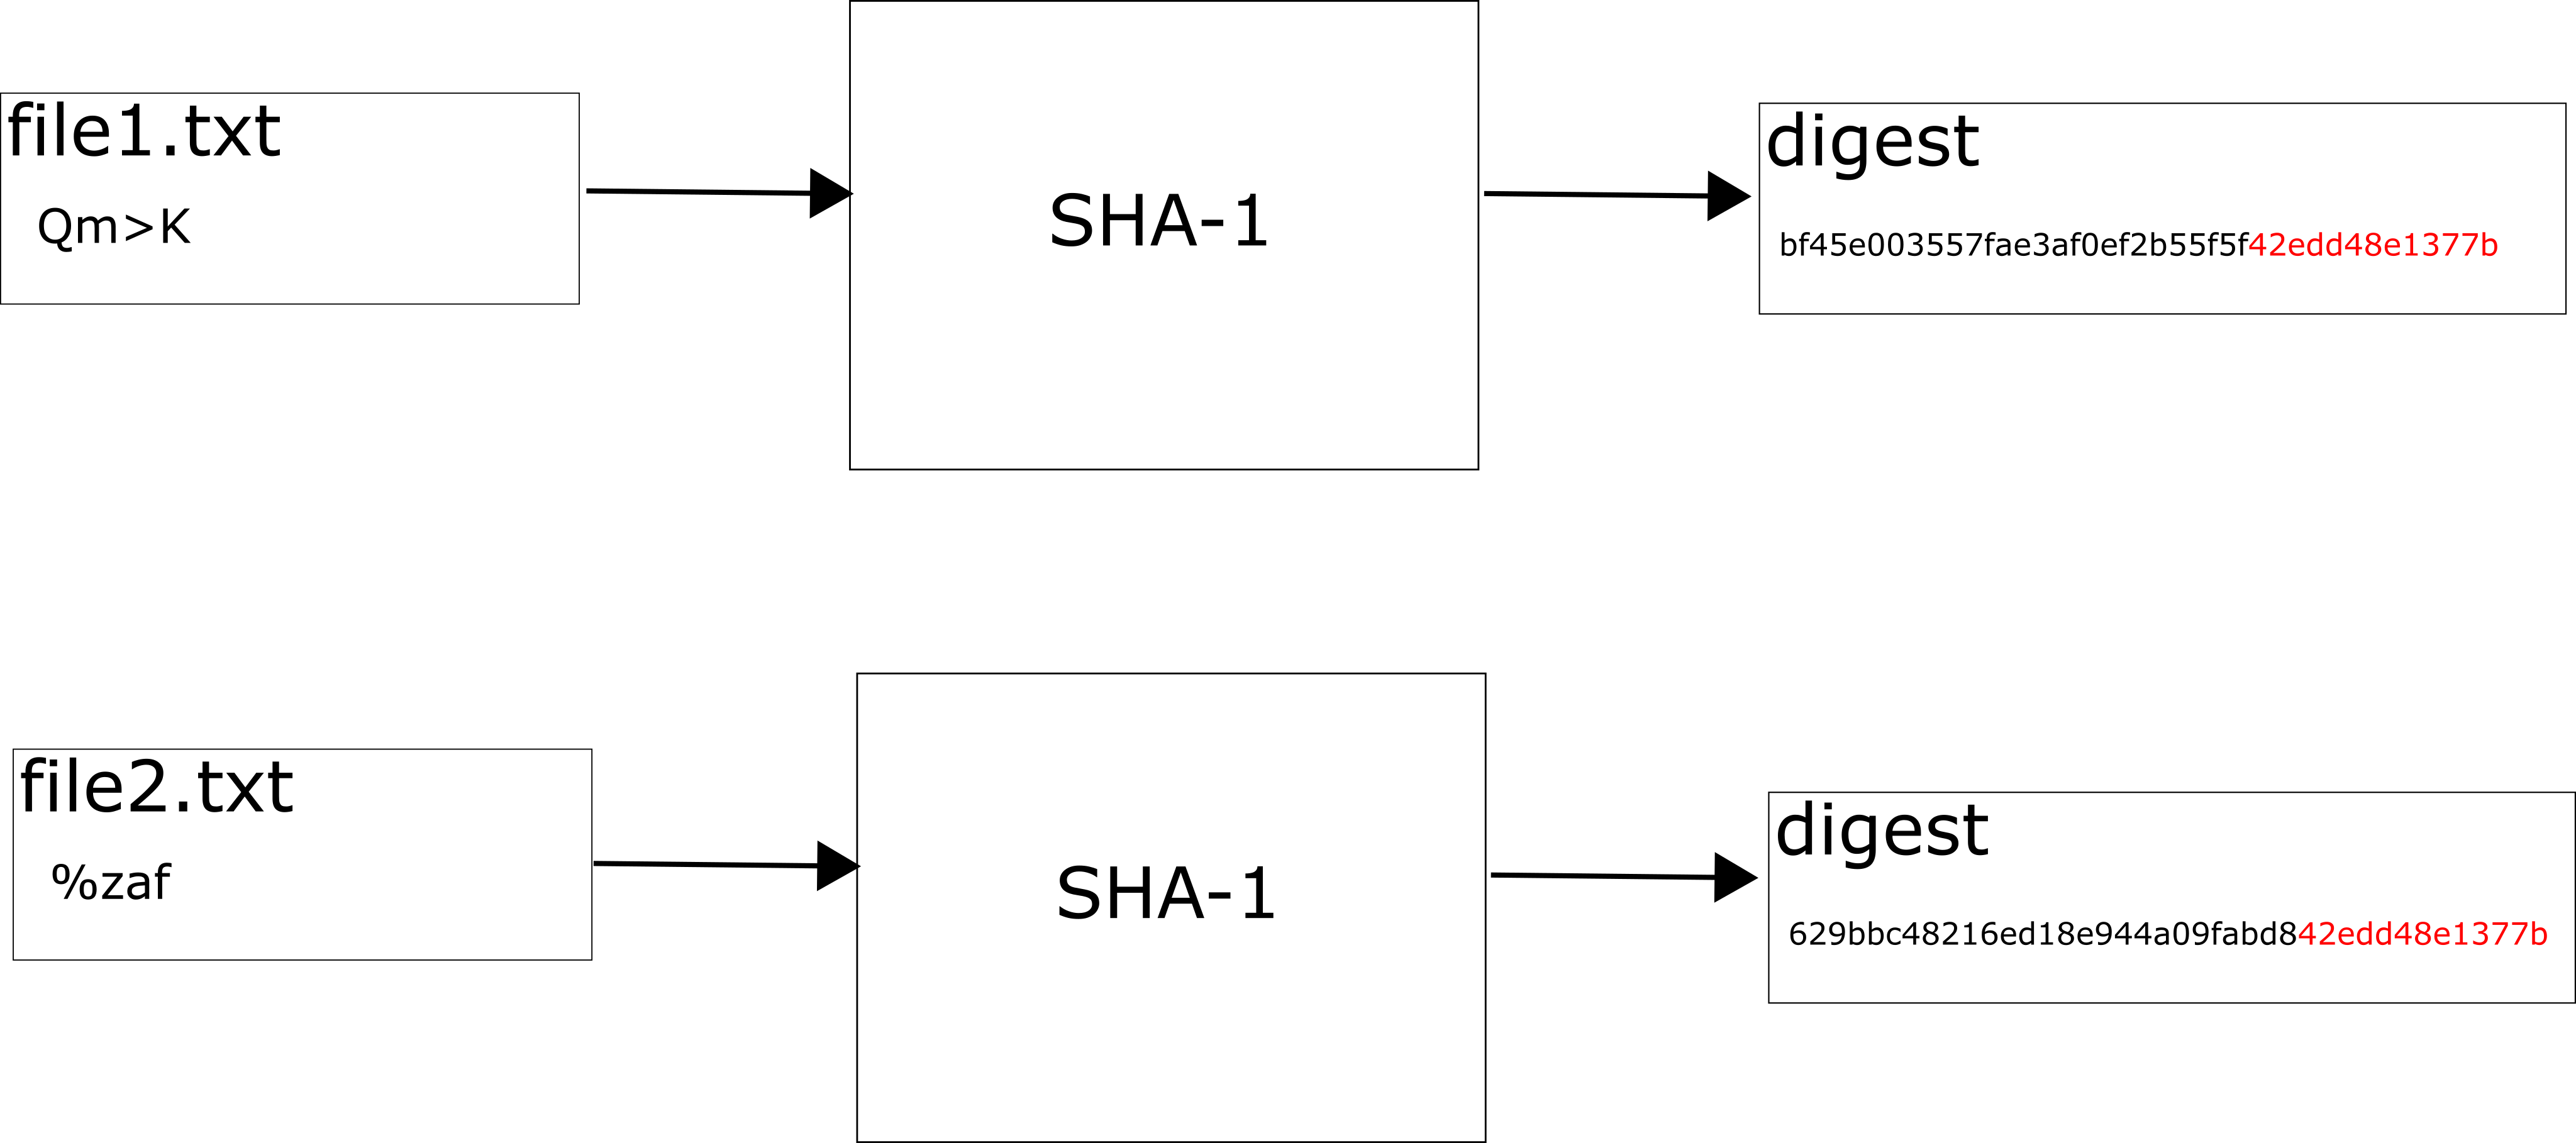
\includegraphics[width=0.6\textwidth]{collision-hw2-1699981.png} % adjust width
	\caption{\textit{Example of collision on weakened SHA-1. The digests above are represented in hexadecimal.}} % optional
	\label{fig:collision}
\end{figure}

\subsection{Memory issues}
I've run the script on my 8 GB RAM laptop: for k = 52, for instance, the number of digests computed before finding the collision is greater than 67 millions, that is $\approx 2^{26}$ (cfr. the birthday paradox). In order to run the script on values $>$ 52, e.g. 56, I had to slightly change it.

\section{Need for space: a smarter approach}
\textit{The totality is not, as it were, a mere heap, but the whole is something besides the parts} stated Aristotle in his Metaphysics. So, instead of building a huge hash-map of digests, I partitioned the digests set in 16 different sets, each associated to a unique map: each of these maps behaved as an index; in fact, map\_0 contained all the digests whose first 4 bits were 0000, map\_1 contained all the ones with 0001 at first, and so on. The sets of the keys contained in each map were (built to be) disjoint. Since I could not have in main memory all the 16 sets, the script simply made 16 iterations, focusing each time on one specific prefix (map\_index) that was effectively analyzed.

\begin{figure}[!ht]
	\centering % optional
	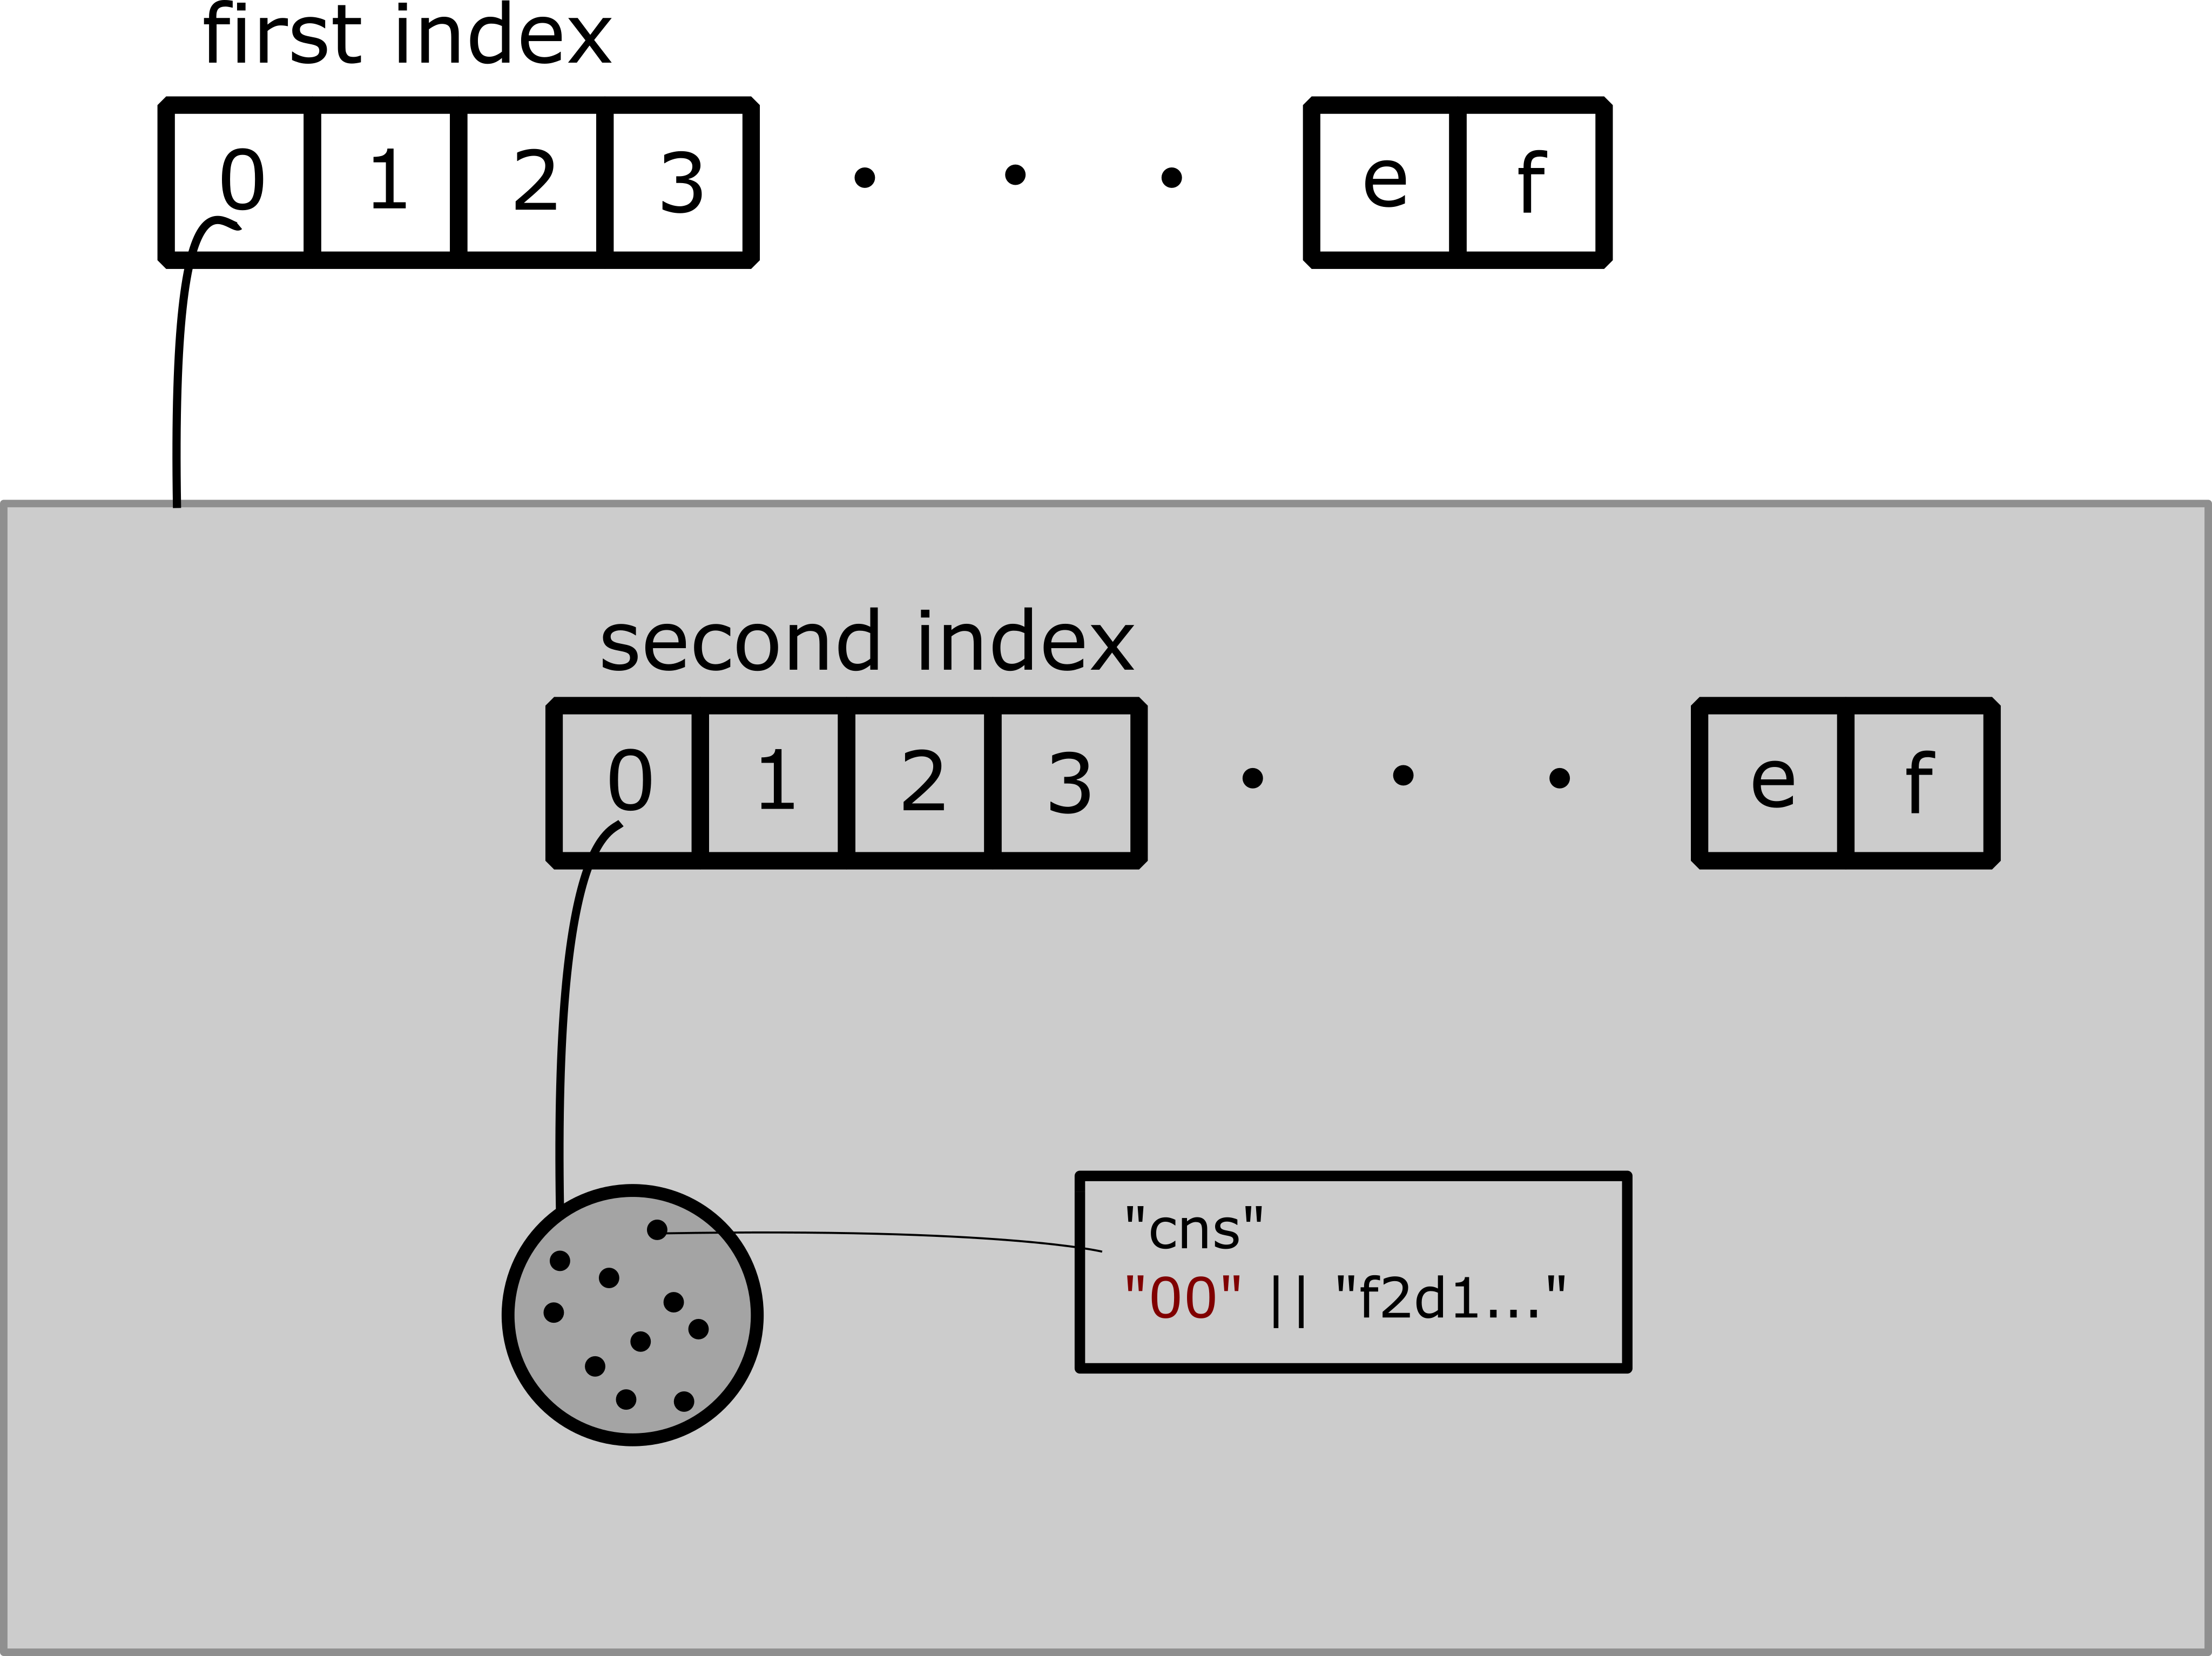
\includegraphics[width=0.6\textwidth]{indexing-hw2-1699981.png} % adjust width
	\caption{\textit{Simple schema of the double indexing used to handle multiple hash-maps. The string in red, i.e. the prefix, is not stored of course because unnecessary.}} % optional
	\label{fig:indexing}
\end{figure}

\subsection{Time complexity and parallelization}
Partitioning the digests set in 16 disjoint sets  is \textit{asymptotically} irrelevant for the time complexity of the algorithm, since 16 is a multiplicative constant that I had to pay (in my trade-off with RAM usage) in order to achieve the goal. Moreover, due the fact that each iteration is independent from the others (because each one searches the collision with a specific pattern) it is possible to parallelize the jobs: e.g given 16 laptops, each of these can process a specific prefix (i.e. the first 4 bits of digests).

\section{Floyd's algorithm}
Even the modified version of the Naive Algorithm requires a lot of RAM to run for very big values of k. For this reason I've decided to adopt a well-known algorithm able to detect a cycle in a graph: the Floyd's algorithm. It requires constant usage of RAM and after a number of iterations ($\approx 2^{k/2}$) converges and finds the collision. I've implemented this algorithm in Python 3, and I've been able to find a collision for k = 66 bits.

\section{Results}
\subsection{Main goal}
I've managed to generate two files with same weakened SHA-1, with \textbf{k = 66}. The files are attached to this report, as file1.txt and file2.txt. In the next table there is a summary of the results obtained  with each method and the resources needed to reach the goal.

\begin{table}[!h]
	\begin{center}
		\begin{tabular}{| l | c | c | c |}
			\hline
			& k & RAM peak (MB) & Iterations (M) \\
			\hline
			Naive & 52 & $\approx$ 4000 & $\approx$ 67 \\
			\hline	
			Modified Naive & 56 & $\approx$ 3000 & $\approx$ 500 \\
			\hline	
			Floyd & \textbf{66} & $<$ 20 & $\approx$ 1300 \\
			\hline	
		\end{tabular}
		\caption{\textit{Results and resource usage for each method.}}
		\label{table:1}
	\end{center}
\end{table}

\subsection{Other considerations}
To be honest, finding the collision with k = 66, was only one of the steps of the script. Indeed, the algorithm can brute-force whatever value: for completeness I've attached the file collisions.txt, where it is possible to find collisions for k $\in$ \{4,8,12,16,20,24,28,32,36,40,44,48,52,56,60,64,66\}: each row reports the number k used, the two words whose digests collide, and the number of digests computed before finding the collision.

\begin{figure}[!ht]
	\centering % optional
	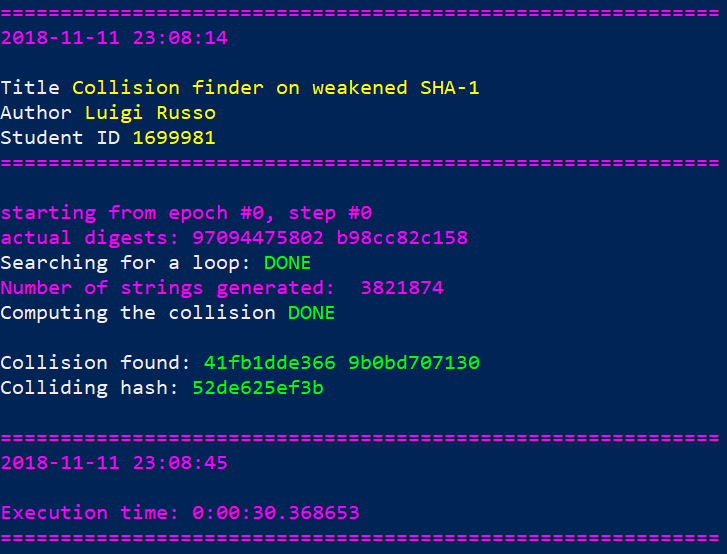
\includegraphics[width=0.7\textwidth]{example-hw2-1699981.png} % adjust width
	\caption{\textit{Example of run, with k = 44.}} % optional
	\label{fig:example}
\end{figure}

\end{document}
